\documentclass[10pt]{article}

% Math environment, symbols, bbm fonts, doublestroke fonts, physics for partial derivatives (pdv{}{})
\usepackage{amsmath,amssymb,bbm,dsfont,physics}
% Define plim operator
\DeclareMathOperator*{\plim}{plim}
% Page size and margins
\usepackage{geometry}
\geometry{letterpaper,tmargin=1in,bmargin=1in,lmargin=1in,rmargin=1in}
% Line spacing
\usepackage{setspace}
\setstretch{1.5} % 1 for default line spacing, 2 for double, etc.
% Hyperlink environment
\usepackage{hyperref}
\hypersetup{colorlinks,linkcolor=red,urlcolor=blue,citecolor=red}
% Table environment
\usepackage{booktabs}
% Threeparttable environment
\usepackage[flushleft]{threeparttable}
% Graphic environment
\usepackage{graphicx}
% Allows float options (e.g. [H] or [!ht])
\usepackage[capposition=top]{floatrow}
% Indents First Paragraph
\usepackage{indentfirst}
% Bibliography with AER style
\usepackage{natbib}
\bibliographystyle{aer}

% Custom section/subsection formatting
\usepackage{titlesec}
% Make section be arabic
\renewcommand{\thesection}{\arabic{section}}
% Make subsection be arabic
\renewcommand{\thesubsection}{\thesection.\arabic{subsection}}
% Make subsubsections be arabic
\renewcommand{\thesubsubsection}{\thesubsection.\arabic{subsubsection}}
% Section title formatting
\titleformat{\section}%
   {\flushleft\bfseries\LARGE}{\thesection}{0.5em}{}
% Subsection title formatting
\titleformat{\subsection}%
   {\Large\bfseries}{\thesubsection}{0.5em}{}
% Subsubsection title formatting
\titleformat{\subsubsection}%
          {\large\bfseries}{\thesubsubsection}{0.5em}{}
% Paragraph title formatting
\setcounter{secnumdepth}{4}
\titleformat{\paragraph}%
          {\large\bfseries}{\theparagraph \newline}{0.5em}{}
% Bibliography title formatting
% Bibliography doesn't using \section*
\renewcommand{\bibsection}{%
   \newpage
   \flushleft{\LARGE{\textbf{{\refname}%
   }}}
}

% Equations numbered by section/subsection
\numberwithin{equation}{subsection}
% No more . inside of equation tags, instead say eqn.
\renewcommand{\theequation}{\thesubsection \text{ eqn.} \arabic{equation}}

% Automatically label sections
\usepackage{letltxmacro}
\LetLtxMacro{\oldsection}{\section}
\renewcommand{\section}[2][]{\oldsection[#1]{#2}\index{#1}\label{sec:\thesection}}
\LetLtxMacro{\oldsubsection}{\subsection}
\renewcommand{\subsection}[2][]{\oldsubsection[#1]{#2}\index{#1}\label{sec:\thesubsection}}
\LetLtxMacro{\oldsubsubsection}{\subsubsection}
\renewcommand{\subsubsection}[2][]{\oldsubsubsection[#1]{#2}\index{#1}\label{sec:\thesubsubsection}}

% Automatically label equations
\LetLtxMacro{\oldequation}{\equation}
\renewcommand{\equation}[2][]{\oldequation{#2}\label{eq:\thesubsection-\arabic{equation}}}
% Automatically label align
\LetLtxMacro{\oldalign}{\align}
\renewcommand{\align}[2][]{\oldalign{#2}\label{eq:\thesubsection-\arabic{equation}}}
% Multiline equations, plus automatically label them
\usepackage{breqn}
\LetLtxMacro{\olddmath}{\dmath}
\renewcommand{\dmath}[2][]{\olddmath{#2}\label{eq:\thesubsection-\arabic{equation}}}

% autoref prints sections/subsections as Section
\renewcommand{\sectionautorefname}{Section}
\renewcommand{\subsectionautorefname}{Section}
\renewcommand{\subsubsectionautorefname}{Section}

% Custom page numbering
\usepackage{fancyhdr,lastpage}
\pagestyle{fancy}
\lfoot{\footnotesize\textsl{Section \ref{sec:1} - \ref{sec:2} - \ref{sec:3} - \hyperref[sec:A]{Appendix}}}
\rfoot{\footnotesize\textsl{Page \thepage\ of \pageref{LastPage}}}
\lhead{} % Remove filler
\chead{} % Remove filler
\rhead{} % Remove filler
\cfoot{} % Remove default page number
\renewcommand\headrulewidth{0pt} % Remove top line

% Appendix autoref
\usepackage{appendix}
\newcommand{\aref}[1]{\hyperref[#1]{Appendix~\ref{#1}}}

% Suppress underfull \hbox warning
\hbadness=10000

% Custom enumerate
\renewcommand{\theenumi}{\alph{enumi}}

% Result dir
\newcommand*{\FigureDir}{../../graphs}
\newcommand*{\DemoDir}{../../code/Rick/OUTPUT/Demographics}
\newcommand*{\SSDir}{../../code/Rick/OUTPUT/SS}
\newcommand*{\TPDir}{../../code/Rick/OUTPUT/TP}

% Colors
\usepackage{xcolor}
\newcommand{\red}{\color{red}}
\newcommand{\blue}{\color{blue}}

% Subfigures
\usepackage{subcaption}

% Footnotes
\usepackage[bottom]{footmisc}

\begin{document}

% %%%%%%%%%%%%%%%%%%%%%%%%%%%%%%%%%%%%%%%%%%%%%%%%%
% \section{EXAMPLE USAGE OF FIGURE AND TABLE}
% %%%%%%%%%%%%%%%%%%%%%%%%%%%%%%%%%%%%%%%%%%%%%%%%%

% FIGURES

% \begin{figure}[H]
%    \centering
%    \caption{\label{fig:p\thesubsection}\autoref{sec:p\thesubsection}}
%    \scalebox{1}{
%       \begin{threeparttable}
%          \begin{tabular}{cc}
%             \includegraphics[width=0.50\textwidth]{\FigureDir/} &
%             \includegraphics[width=0.50\textwidth]{\FigureDir/} \\
%             \includegraphics[width=0.50\textwidth]{\FigureDir/} &
%             \includegraphics[width=0.50\textwidth]{\FigureDir/}
%          \end{tabular}
%       \end{threeparttable}
%    }
% \end{figure}

% SIDE BY SIDE FIGURES WITH CAPTIONS

% \begin{figure}[H]
%    \caption{\label{fig:\thesubsubsection1}}
%    \begin{subfigure}{0.5\textwidth}
%       \centering
%       \includegraphics[width=\textwidth]{\SSDir/static/images/SS_n.png}
%       \caption{Subfig 1}
%    \end{subfigure}% <-- this "%" symbol is important
%    ~ % <-- this "~" symbol is important
%    \begin{subfigure}{0.5\textwidth}
%       \centering
%       \includegraphics[width=\textwidth]{\SSDir/dynamic_partial/images/SS_n.png}
%       \caption{Subfig 2}
%    \end{subfigure}
%    \newline <-- this creates a new lines
%    \begin{subfigure}{0.5\textwidth}
%       \centering
%       \includegraphics[width=\textwidth]{\SSDir/dynamic_full/images/SS_n.png}
%       \caption{Subfig 3}
%    \end{subfigure}%
%    ~ % <-- this "~" symbol is important
%    \begin{subfigure}{0.5\textwidth}
%       \centering
%       \includegraphics[width=\textwidth]{\SSDir/dynamic_full/images/SS_n.png}
%       \caption{Subfig 4}
%    \end{subfigure}
% \end{figure}

% TABLES

% \begin{table}[H]
%    \centering
%    \scalebox{0.75}{
%       \begin{threeparttable}\caption{\label{tab:p\thesubsection}\autoref{sec:p\thesubsection}}
%          \begin{tabular}{lcc}
%             \hline\hline\addlinespace
%             \input{../regression_tables/p1a.tex}
%             \addlinespace\hline\hline
%          \end{tabular}
%          \begin{tablenotes}
%             \item 
%             Standard errors in parentheses.
%          \end{tablenotes}
%       \end{threeparttable}
%    }
% \end{table}

% SIDE BY SIDE TABLES

% \begin{table}[H]
%    \begin{minipage}[t]{0.5\textwidth}
%      PUT TABLE 1 HERE
%    \end{minipage}% <-- this "%" symbol is important
%    \begin{minipage}[t]{0.5\textwidth}
%      PUT TABLE 2 HERE
%    \end{minipage}
% \end{table}

% How to reference sections: \autoref{sec:1}
% How to reference subsections: \autoref{sec:p1a}
% How to reference equations: \ref{eq:1a1} for section 1, subsection a, equation 1

% %%%%%%%%%%%%%%%%%%%%%%%%%%%%%%%%%%%%%%%%%%%%%%%%%
% \section{Thesis}
% %%%%%%%%%%%%%%%%%%%%%%%%%%%%%%%%%%%%%%%%%%%%%%%%%

% %%%%%%%%%%%%%%%%%%%%%%%%%%%%%%%%%%%%%%%%%%%%%%%%%
% \section{Title Page}
% %%%%%%%%%%%%%%%%%%%%%%%%%%%%%%%%%%%%%%%%%%%%%%%%%

\begin{titlepage}
\title{Estimation Effects of Various Demographic Forecasting Techniques in Japan Using an Overlapping Generations Model 
         \thanks{I would like to thank Dr. Richard Evans for the guidance and support he provided while writing my thesis.}
      }
\author{
   Adam Alexander Oppenheimer
   \footnote{University of Chicago,
      Department of Economics. Email:
      \href{mailto:oppenheimer@uchicago.edu}
      {oppenheimer@uchicago.edu}.
   }
}
\date{March 2020 \\
   \scriptsize{}}
\maketitle
\vspace{-9mm}
\begin{abstract}
\small{First paragraph in the abstract
\par Second paragraph in the abstract

\vspace{3mm}

\noindent\textit{keywords:}\:
   Overlapping Generations Model,
   Demographic Transition,
   Japan Calibration

\vspace{3mm}

}

\end{abstract}
\thispagestyle{empty}
\end{titlepage}

% %%%%%%%%%%%%%%%%%%%%%%%%%%%%%%%%%%%%%%%%%%%%%%%%%
% \section{Introduction}
% %%%%%%%%%%%%%%%%%%%%%%%%%%%%%%%%%%%%%%%%%%%%%%%%%

\section{Introduction}

Research question: how does changing the population forecasting model alter future tax revenue through its effect on labor supply?
\\\\
Literature review: primarily building off Kei and my previous paper. That paper uses as inspiration Muto et. al 2016, who carry out an overlapping generations analysis of the effects of these demographic shifts on long-run aggregate outcomes for Japan. They find that decreasing fertility rates contribute to decreasing aggregate output, while increasing longevity counteracts this by increasing aggregate output.  However, this increase is not enough to create a net positive effect. Overall, their simulation predicts negative effects on aggregate outputs during the next few decades.
\\\\
There are many other OLG models looking at the Japanese demographic transition but that is the most recently published paper. These papers almost entirely use the National Institute of Population and Social Security Research fertility/mortality/population forecasts. Some use UN estimates.

% %%%%%%%%%%%%%%%%%%%%%%%%%%%%%%%%%%%%%%%%%%%%%%%%%
% \section{Model}
% %%%%%%%%%%%%%%%%%%%%%%%%%%%%%%%%%%%%%%%%%%%%%%%%%

\section{Model}

Simpler OLG than that used in Kei and my previous paper.

% %%%%%%%%%%%%%%%%%%%%%%%%%%%%%%%%%%%%%%%%%%%%%%%%%
% \section{Data}
% %%%%%%%%%%%%%%%%%%%%%%%%%%%%%%%%%%%%%%%%%%%%%%%%%

\section{Data}

Same data as Kei and my previous paper. Fertility data from the Human Fertility Collection. Mortality and population data from the Japanese Mortality Database. Frisch elasticity of 0.5 from Muto et. al. Wage data by age from Basic Survey on Wage Structure. Labor force participation rates by age from Labour Force Survey. Tax rates from Tax Guide Book.

% %%%%%%%%%%%%%%%%%%%%%%%%%%%%%%%%%%%%%%%%%%%%%%%%%
% \section{Results}
% %%%%%%%%%%%%%%%%%%%%%%%%%%%%%%%%%%%%%%%%%%%%%%%%%

\section{Results}

No OLG results yet. See \autoref{sec:A} for demographic transition forecasts.

% %%%%%%%%%%%%%%%%%%%%%%%%%%%%%%%%%%%%%%%%%%%%%%%%%
% \section{Conclusion}
% %%%%%%%%%%%%%%%%%%%%%%%%%%%%%%%%%%%%%%%%%%%%%%%%%

\section{Conclusion}

Extensions: endogenous fertility.

% %%%%%%%%%%%%%%%%%%%%%%%%%%%%%%%%%%%%%%%%%%%%%%%%%
% \section{Bibliography}
% %%%%%%%%%%%%%%%%%%%%%%%%%%%%%%%%%%%%%%%%%%%%%%%%%

\bibliography{thesis_bib.bib}

% %%%%%%%%%%%%%%%%%%%%%%%%%%%%%%%%%%%%%%%%%%%%%%%%%
% \section{Appendix}
% %%%%%%%%%%%%%%%%%%%%%%%%%%%%%%%%%%%%%%%%%%%%%%%%%

\newpage
\begin{appendices}
\section{Appendix}

% %%%%%%%%%%%%%%%%%%%%%%%%%%%%%%%%%%%%%%%%%%%%%%%%%
% \subsection{Appendix - Model}
% %%%%%%%%%%%%%%%%%%%%%%%%%%%%%%%%%%%%%%%%%%%%%%%%%

\subsection{Overlapping Generations Model}

We use the overlapping generations model described in \cite{E2020}. The model includes households and firms, endogenous labor, and exogenous productivity growth. Demographics are exogenous and fertility, mortality, and immigration rates can evolve over time. As a result of including mortality rates, the model includes unintended bequests. The model also incorporates a warm bequest motive to introduce an implicit borrowing constraint. A detailed description of the model follows.

% %%%%%%%%%%%%%%%%%%%%%%%%%%%%%%%%%%%%%%%%%%%%%%%%%
% \subsubsection{Appendix - Model - Economic Model}
% %%%%%%%%%%%%%%%%%%%%%%%%%%%%%%%%%%%%%%%%%%%%%%%%%

\subsubsection{Overlapping Generations Economic Model}

% %%%%%%%%%%%%%%%%%%%%%%%%%%%%%%%%%%%%%%%%%%%%%%%%%
% \paragraph{Appendix - Model - Households}
% %%%%%%%%%%%%%%%%%%%%%%%%%%%%%%%%%%%%%%%%%%%%%%%%%

\paragraph{Households}

The consumption side of the economy is given by identical households. The measure of all households of age \(s\) in period \(t\) is denoted by \(\omega_{s,t}\). Households live at most \(E+S\) periods and become economically relevant at age \(E+1\). Households are endowed with a measure of time \(\tilde{l}\) to distribute between labor (\(n_{s,t} \in [0,\tilde{l}]\)) and leisure (\(l_{s,t} \in [0,\tilde{l}]\)), where \(n_{s,t} + l_{s,t} = \tilde{l} \hspace{3mm} \forall s, t\). Households then choose consumption \(c_{s,t}\), labor \(n_{s,t}\), and savings \(b_{s+1,t+1}\) to maximize the following utility function:

\begin{dmath}
   {u(c_{s,t}, n_{s,t}, b_{s+1,t+1}) = \frac{(c_{s,t})^{1-\sigma}-1}{1-\sigma} + e^{g_yt(1-\sigma)}\chi_{n,s}b\left[1-\left(\frac{n_{s,t}}{\tilde{l}}\right)\right]^{\frac{1}{\upsilon}}} \\
   {\hspace{40mm} + \rho_{s,t}\chi_b\frac{(b_{s+1,t+1})^{1-\sigma}-1}{1-\sigma} \hspace{3mm} \forall s,t}
\end{dmath}

\par subject to the following constraint:

\begin{equation}
   c_{s,t} + b_{s+1,t+1} = (1+r_t)b_{s,t} + w_tn_{s,t} + \frac{BQ_t}{\tilde{N}_t} \hspace{3mm} \forall t \hspace{3mm} \text{and} \hspace{3mm} s \geq E+1
\end{equation}

\par In the utility function, the utility of consumption is CRRA and is given by the first term on the right hand side; labor is subject to elliptical disutility as described in \cite{DE2018} and is given by the second term on the right hand side; and the warm bequest motive is given by the third term on the right hand side. We assume that savings upon entering the workforce and in the last possible period of life are zero (\(b_{E+1,t} = b_{E+S+1,t} = 0\)) and that \(c_{s,t} \geq 0\) (this results in \(c_{s,t} > 0\) in equilibrium).

\par In the elliptical disutility of labor term, \(e^{g_yt(1-\sigma)}\) scales the utility of labor to be in units comparable to the utility of consumption. This is necessary because labor is stationary but consumption is non-stationary, meaning that their unscaled utility measures are not comparable over time. The remaining variables in the elliptical disutility of labor term are defined in \cite{DE2018}.

\par In the warm bequest motive term, \(\rho_{s,t}\) gives the probability of dying at age \(s\) in time \(t\) and \(\chi_b\) gives a warm bequest motive parameter necessary for fitting data moments. The warm bequest motive provides utility for dying with positive savings. This implicitly introduces a borrowing constraint at zero, as the marginal utility of savings becomes infinity at zero savings by the Inada condition on this term.

\par In the budget constraint, \(BQ_t\) gives the total sum of unintended bequests left by the population that died in the previous period.\footnote{We formally define bequests as \(BQ_t = (1+r_t)\sum_{s=E+2}^{E+S+1}\rho_{s-1,t-1}\omega_{s-1,t-1}b_{s,t} \hspace{3mm} \forall t\)} This is divided by \(\tilde{N}_t\) to ensure bequests are evenly distributed among the economically relevant population. We define \(r_t\) and \(w_t\) as the interest rate and wage in period \(t\), respectively.

\par Further detail about solving the household's problem, such as deriving the first order conditions, solving the Euler equations, and solving the optimal paths of labor supply and savings given initial savings and the time paths of factor prices and total bequests can be read in \cite{E2020}.

% %%%%%%%%%%%%%%%%%%%%%%%%%%%%%%%%%%%%%%%%%%%%%%%%%
% \paragraph{Appendix - Model - Firms}
% %%%%%%%%%%%%%%%%%%%%%%%%%%%%%%%%%%%%%%%%%%%%%%%%%

\paragraph{Firms}

The production side of the economy is given by a unit measure of identical, perfectly competitive firms. Firms produce following a Cobb-Douglas production function as follows:

\begin{equation}
   Y_t = F(K_t, L_t) \equiv A(K_t)^\alpha(e^{g_yt}L_t)^{1-\alpha} \forall t \hspace{3mm} \alpha \in (0, 1) \hspace{3mm} \text{and} \hspace{3mm} A>0
\end{equation}

\par where \(A\) gives the level of technology, \(K_t\) gives capital, \(L_t\) gives labor, \(\alpha\) gives the fraction of spending on capital relative to labor, and \(g_y\) gives the growth rate of labor productivity over time.

\par Firms maximize the following profit function:

\begin{equation}
   PR_t = A(K_t)^\alpha(e^{g_yt}L_t)^{1-\alpha} - (r_t + \delta)K_t - w_tL_t \hspace{3mm} \forall t
\end{equation}

\par where firms choose \(K_t\) and \(L_t\), and \(\delta \in [0, 1]\) gives the rate of capital depreciation. Solving the first order conditions by taking derivatives with respect to capital and labor allows us to characterize the firm's optimal behavior as the following:

\begin{align}
   r_t = \alpha\left(\frac{Y_t}{K_t}\right) - \delta \hspace{3mm} \forall t \\
   w_t = (1-\alpha)\left(\frac{Y_t}{L_t}\right)\hspace{3mm} \forall t
\end{align}

% %%%%%%%%%%%%%%%%%%%%%%%%%%%%%%%%%%%%%%%%%%%%%%%%%
% \paragraph{Appendix - Model - Market Clearance}
% %%%%%%%%%%%%%%%%%%%%%%%%%%%%%%%%%%%%%%%%%%%%%%%%%

\paragraph{Market Clearance}

The model we consider includes three markets that must clear: the labor market, the capital market, and the goods market. By Walras' Law, we need only consider the clearance of two of these markets in order for all three to clear. The three markets clearing conditions are as follows:

\textbf{Labor Market:}
\begin{equation}
   L_t = \sum_{s=E+1}^{E+S}\omega_{s,t}n_{s,t}
\end{equation}

\textbf{Capital Market:}
\begin{equation}
   K_t = \sum_{s=E+2}^{E+S+1}\Bigl(\omega_{s-1,t-1}b_{s,t}+i_{s,t}\omega_{s,t-1}b_{s,t}\Bigr)
\end{equation}

\textbf{Goods Market:}
\begin{dmath}
   Y_t = C_t + I_t - \sum_{s=E+2}^{E+S+1}i_{s,t+1}\omega_{s,t}b_{s,t+1} \\
   {\text{where} \hspace{3mm} I_t \equiv K_{t+1} - (1-\delta)K_t} \\
   {\text{and} \hspace{3mm} C_t \equiv \sum_{s=E+1}^{E+S}\omega_{s,t}c_{s,t}}
\end{dmath}

\par It is important to note that immigration is included in the capital and goods market clearing equations. This implies that capital held by immigrants goes into production in Japan and the capital held by emigrants leaves production in Japan. The last term in the goods market clearing equation represents net exports in this model.\footnote{In general, this would represent the capital account portion of net exports.} It should be noted that we assume that the capital held by immigrant households is equal to the capital held by equivalent households within Japan.

% %%%%%%%%%%%%%%%%%%%%%%%%%%%%%%%%%%%%%%%%%%%%%%%%%
% \paragraph{Appendix - Model - Stationarization and Equilibrium}
% %%%%%%%%%%%%%%%%%%%%%%%%%%%%%%%%%%%%%%%%%%%%%%%%%

\paragraph{Stationarization and Equilibrium}

Please refer to \cite{E2020} for a detailed description of how to stationarize the model and solve the equilibrium.

% %%%%%%%%%%%%%%%%%%%%%%%%%%%%%%%%%%%%%%%%%%%%%%%%%
% \subsubsection{Appendix - Model - Demographics}
% %%%%%%%%%%%%%%%%%%%%%%%%%%%%%%%%%%%%%%%%%%%%%%%%%

\subsubsection{Demographics}

We consider four demographic models. The first model assumes that demographics are constant over time. The second, third, and fourth models use the methods described in the following section to solve the steady state level of demographics. The second model assumes that fertility, mortality, and immigration are at their 2019 levels. The third model uses a parametric method described in \autoref{sec:A.2} to forecast fertility, mortality, and immigration over time. The fourth model uses the \(R\) package Demographics (\cite{alt_demo}) to forecast fertility, mortality, and immigration over time using principal components analysis. For the second third, and fourth models, population evolution follows \ref{eq:A.2-1}, where the \(s\) subscript indicates age and the \(t\) subscript indicates period. \(\omega_{s,t}, f_{s,t}, \rho_{s,t} \geq 0\) represent the age- and period-specific population, fertility rate, and mortality rate. \(i_{s,t}\) represents the net immigration rate. Agents live for a maximum of \(E+S\) periods, where \(S \geq 3\) and \(E + 1\) indicates the first working year of life. Agents age \(\leq E\) are modeled in population dynamics but are considered outside the economy. Population and mortality rate data comes from \cite{JMD2018}. Fertility rate data comes from \cite{HFC2018}.

\begin{dmath}
   {\omega_{1,t+1} = (1 - \rho_{0,t})\sum_{s=1}^{E+S}f_{s,t}\omega_{s,t} + i_{1,t}\omega_{1,t} \hspace{3mm} \forall t} \\
   {\omega_{s+1,t+1} = (1 - \rho_{s,t})\omega_{s,t} + i_{s+1,t}\omega_{s+1,t} \hspace{3mm} \forall t \hspace{3mm} \text{and} \hspace{3mm} 1 \leq s \leq E + S - 1}
\end{dmath}

\par This is a slight variation on the model used by \cite{DE2018} and \citet{IO2019}. The model used in both these papers assumes fertility, mortality and immigration rates are fixed at their 2014 levels. This paper attempts to forecast changes in those variables over time.

\par We now define some variables that are relevant to the remaining model sections. \(N_t\) gives the total population. \(g_{n,t}\) gives the population growth rate from period \(t-1\) to period \(t\). A variable accented by \(\sim\) indicates that is defined for only the working age population. The formal definitions of these variables follow.

\begin{align}
   N_t \equiv \sum_{s=1}^{E+S}\omega_{s,t} \hspace{3mm} \forall t \\
   g_{n,t+1} \equiv \frac{N_{t+1}}{N_t} - 1 \hspace{3mm} \forall t \\
   \tilde{N}_t \equiv \sum_{s=E+1}^{E+S}\omega_{s,t} \hspace{3mm} \forall t \\
   \tilde{g}_{n,t+1} \equiv \frac{\tilde{N}_{t+1}}{\tilde{N}_t} - 1 \hspace{3mm} \forall t
\end{align}

% %%%%%%%%%%%%%%%%%%%%%%%%%%%%%%%%%%%%%%%%%%%%%%%%%
% \paragraph{Appendix - Model - Fertility, Mortality, and Immigration Rates}
% %%%%%%%%%%%%%%%%%%%%%%%%%%%%%%%%%%%%%%%%%%%%%%%%%

\paragraph{Fertility, Mortality, and Immigration Rates}

In order to allow for a range of model years, we fit fertility and mortality rates using cubic spline interpolation. The fit of the interpolated data to the real data can be seen in \autoref{fig:\thesubsubsection1}. In this case, the fertility data is for all ages 14 to 50, and we impute fertility rates of 0 for all other ages; while the mortality data is for all ages from 0 to 99, and we set mortality to 1 at age 99. The interpolated function is fit at the midpoints of the data. It should exactly overlay the midpoint of the trend in the data, as it does. While in this case we consider only 1-year bins, the model allows for any positive bin size through the use of population-weighted fertility and mortality rates.

\begin{figure}[H]
   \caption{\label{fig:\thesubsubsection1}Fertility and Mortality Rates by Age}
   \begin{subfigure}{0.5\textwidth}
      \centering
      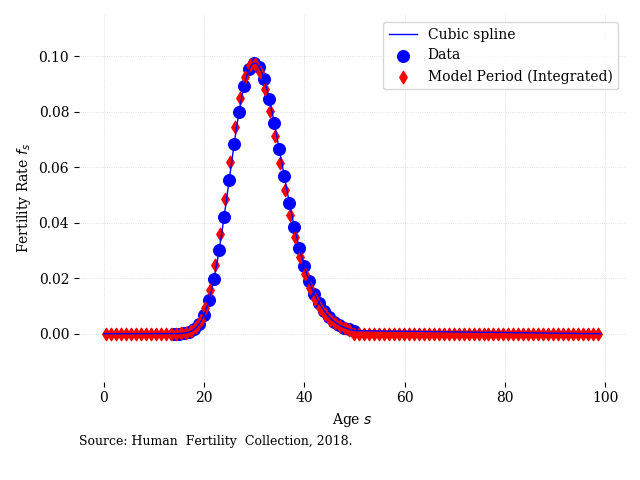
\includegraphics[width=\textwidth]{\DemoDir/fert_rates.png}
      \caption{Japanese Fertility Rates by Age (2020, Forecasted)}
   \end{subfigure}% <-- this "%" symbol is important
   ~ % <-- this "~" symbol is important
   \begin{subfigure}{0.5\textwidth}
      \centering
      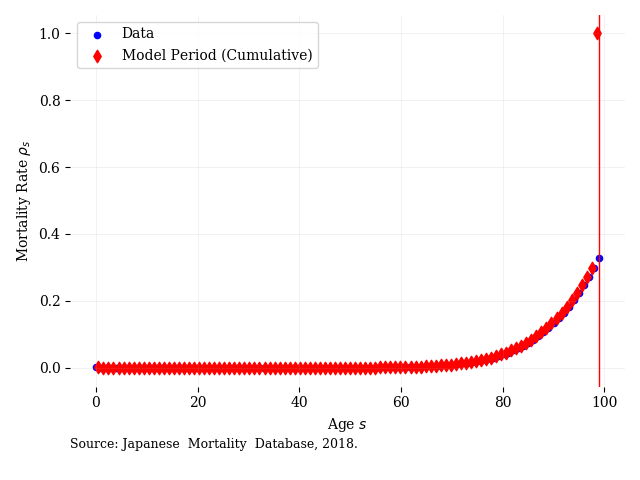
\includegraphics[width=\textwidth]{\DemoDir/mort_rates.png}
      \caption{Japanese Mortality Rates by Age (2020, Forecasted)}
   \end{subfigure}
\end{figure}

\par Because accurate age-specific immigration rate data is not available for Japan, we estimate it as the residual between predicted and true population from \ref{eq:A.1-1}. The formal definition of immigration rates can be seen in \ref{eq:A.1-6}.

\begin{dmath}
   {i_{1,t+1} = \frac{\omega_{1,t+1} - (1-\rho_{0,t})\sum_{s=1}^{E+S}f_{s,t}\omega_{s,t}}{\omega_{1,t}} \hspace{3mm} \forall t} \\
   {i_{s+1,t+1} = \frac{\omega_{s+1,t+1} - (1-\rho_{0,t})\omega_{s,t}}{\omega_{s+1,t}} \hspace{3mm} \forall t \hspace{3mm} \text{and} \hspace{3mm} 1 \leq s \leq E + S - 1}
\end{dmath}

% %%%%%%%%%%%%%%%%%%%%%%%%%%%%%%%%%%%%%%%%%%%%%%%%%
% \paragraph{Appendix - Model - Population Steady State and Transition Path}
% %%%%%%%%%%%%%%%%%%%%%%%%%%%%%%%%%%%%%%%%%%%%%%%%%

\paragraph{Population Steady State and Transition Path}

\cite{E2020} proves that so long as the fertility, mortality, and immigration rates stabilize at some time \(T\), we can solve for the unique eigenvalue and eigenvector of the matrix representation of the population evolution equation. This eigenvalue can be represented as \((1 + \overline{g}_n)\), where \(\overline{g}_n\) gives the steady state population growth rate. In order to ensure that the population reaches its steady state more quickly, we artificially force the population to achieve its steady state value at \(t=120\). This is achieved by a slight adjustment of immigration rates. Steady state population, adjusted immigration rates, and the population transition path for the four demographic models we consider can be seen in \autoref{fig:A.1.2.1}.

\begin{figure}[!ht]
   \centering
   \caption{\label{fig:\thesubsubsection.1}Population Steady State, and Adjustments, and Transition Path}
   \textbf{Static Demographics}
   \begin{subfigure}{0.33\textwidth}
      \centering
      \includegraphics[width=\textwidth]{\DemoDir/static/OrigVsFixSSpop.png}
   \end{subfigure}% <-- this "%" symbol is important
   ~ % <-- this "~" symbol is important
   \begin{subfigure}{0.33\textwidth}
      \centering
      \includegraphics[width=\textwidth]{\DemoDir/static/OrigVsAdjImm.png}
   \end{subfigure}% <-- this "%" symbol is important
   ~ % <-- this "~" symbol is important
   \begin{subfigure}{0.33\textwidth}
      \centering
      \includegraphics[width=\textwidth]{\DemoDir/static/PopDistPath.png}
   \end{subfigure}

   \textbf{Partial-Dynamic Demographics}
   \begin{subfigure}{0.33\textwidth}
      \centering
      \includegraphics[width=\textwidth]{\DemoDir/dynamic_partial/OrigVsFixSSpop.png}
   \end{subfigure}% <-- this "%" symbol is important
   ~ % <-- this "~" symbol is important
   \begin{subfigure}{0.33\textwidth}
      \centering
      \includegraphics[width=\textwidth]{\DemoDir/dynamic_partial/OrigVsAdjImm.png}
   \end{subfigure}% <-- this "%" symbol is important
   ~ % <-- this "~" symbol is important
   \begin{subfigure}{0.33\textwidth}
      \centering
      \includegraphics[width=\textwidth]{\DemoDir/dynamic_partial/PopDistPath.png}
   \end{subfigure}

   \textbf{Full-Dynamic Demographics}
   \begin{subfigure}{0.33\textwidth}
      \centering
      \includegraphics[width=\textwidth]{\DemoDir/dynamic_full/OrigVsFixSSpop.png}
   \end{subfigure}% <-- this "%" symbol is important
   ~ % <-- this "~" symbol is important
   \begin{subfigure}{0.33\textwidth}
      \centering
      \includegraphics[width=\textwidth]{\DemoDir/dynamic_full/OrigVsAdjImm.png}
   \end{subfigure}% <-- this "%" symbol is important
   ~ % <-- this "~" symbol is important
   \begin{subfigure}{0.33\textwidth}
      \centering
      \includegraphics[width=\textwidth]{\DemoDir/dynamic_full/PopDistPath.png}
   \end{subfigure}

   \textbf{Alternate Full-Dynamic Demographics}
   \begin{subfigure}{0.33\textwidth}
      \centering
      \includegraphics[width=\textwidth]{\DemoDir/dynamic_full_alternate/OrigVsFixSSpop.png}
      \caption{\\ \shortstack{Original vs. Adjusted\\SS Population Distribution}}
   \end{subfigure}% <-- this "%" symbol is important
   ~ % <-- this "~" symbol is important
   \begin{subfigure}{0.33\textwidth}
      \centering
      \includegraphics[width=\textwidth]{\DemoDir/dynamic_full_alternate/OrigVsAdjImm.png}
      \caption{\\ \shortstack{Original vs. Adjusted\\Immigration Rates}}
   \end{subfigure}% <-- this "%" symbol is important
   ~ % <-- this "~" symbol is important
   \begin{subfigure}{0.33\textwidth}
      \centering
      \includegraphics[width=\textwidth]{\DemoDir/dynamic_full_alternate/PopDistPath.png}
      \caption{\\ \shortstack{Population Distribution\\Along Time Path}}
   \end{subfigure}
\end{figure}

% %%%%%%%%%%%%%%%%%%%%%%%%%%%%%%%%%%%%%%%%%%%%%%%%%
% \subsection{Appendix - Dynamic Demographics}
% %%%%%%%%%%%%%%%%%%%%%%%%%%%%%%%%%%%%%%%%%%%%%%%%%

\subsection{Dynamic Demographics}

The following sections discuss calibration and estimation for a parametric method to forecast fertility rates, mortality rates, immigration rates, and population.

% %%%%%%%%%%%%%%%%%%%%%%%%%%%%%%%%%%%%%%%%%%%%%%%%%
% \subsubsection{Appendix - Demographics - Fertility Rates}
% %%%%%%%%%%%%%%%%%%%%%%%%%%%%%%%%%%%%%%%%%%%%%%%%%

\subsubsection{Fertility Rates}

I begin the fertility rate estimation by fitting the yearly distributions using a generalized beta 2 distribution. The pdf for this distribution can be seen in \ref{eq:A.1-3}:

\begin{equation}
   f(x|a, b, p, q) = \frac{ax^{ap-1}}{b^{ap}B(p,q)\left(1 + \left(\frac{x}{b}\right)^a\right)^{p+q}}, \hspace{5mm} x \in [0,\infty); a, b, p, q > 0   
\end{equation}

\noindent
where \(B(v,w) = \int_0^1 t^{v-1}(1-t)^{w-1}dt\) is the beta function. Because the generalized beta 2 is a pdf but fertility rates are not a pdf, I also have to add in a scale parameter. I estimate fertility parameters from 1970 to 2014, the most recent year of data. I chose to begin in 1970 because the most recent trend in data seems to have started around then.
\\\\
The fit of the model in selected years can be seen in \autoref{fig:\thesubsubsection1}. The fit at the peak of the distribution is very close. The fit at the tails of the distribution is good at first but weakens over time - while it is possible to estimate parameters that better fit the tail for more recent data, the variance of the parameter estimates grows considerably and a trend in parameters disappears. Because of this, I chose to use parameters that had a slightly worse fit to the data in order to better estimate a trend.

\begin{figure}[!ht]
   \centering
   \caption{\label{fig:\thesubsubsection1}Fertility Estimated by Generalized Beta 2}
   \scalebox{0.9}{
      \begin{threeparttable}
         \begin{tabular}{cc}
            \includegraphics[width=0.50\textwidth]{\FigureDir/fertility/smooth_0/1970.png} &
            \includegraphics[width=0.50\textwidth]{\FigureDir/fertility/smooth_0/1990.png} \\
            \includegraphics[width=0.50\textwidth]{\FigureDir/fertility/smooth_0/2000.png} &
            \includegraphics[width=0.50\textwidth]{\FigureDir/fertility/smooth_0/2014.png}
         \end{tabular}
      \end{threeparttable}
   }
\end{figure}

\noindent
Parameter estimates and their fit over time can be seen in \autoref{fig:\thesubsubsection2}. In order to ensure estimated trends converge over time, I fit these parameter estimates to logistic functions. The logistic function can be seen in \ref{eq:A.1-4}:

\begin{equation}
   f(x|L, k, x_0) = \frac{L}{1 + e^{-k(x-x_0)}}
\end{equation}

\noindent
where \(L\) represents the maximum value of the curve, \(k\) represents the steepness of the curve, and \(x_0\) represents the midpoint of the curve.

\begin{figure}[H]
   \centering
   \caption{\label{fig:\thesubsubsection2}Fertility Generalized Beta 2 Parameter Estimates}
   \scalebox{0.9}{
      \begin{threeparttable}
         \begin{tabular}{cc}
            \includegraphics[width=0.50\textwidth]{\FigureDir/fertility/smooth_0/_a_predicted.png} &
            \includegraphics[width=0.50\textwidth]{\FigureDir/fertility/smooth_0/_b_predicted.png} \\
            \includegraphics[width=0.50\textwidth]{\FigureDir/fertility/smooth_0/_p_predicted.png} &
            \includegraphics[width=0.50\textwidth]{\FigureDir/fertility/smooth_0/_q_predicted.png}
         \end{tabular}
      \end{threeparttable}
   }
   \scalebox{0.9}{
      \begin{tabular}{ccc}
         & \includegraphics[width=0.50\textwidth]{\FigureDir/fertility/smooth_0/_scale_predicted.png} &
      \end{tabular}
   }
\end{figure}

\noindent
With the parameters from the logistic function estimated, we can now test the quality of our model fit. Comparisons of the models estimated with true data can be seen in \autoref{fig:\thesubsubsection3}. The first panel shows the trend in true fertility rates from 1970-2014; the second panel shows the trend in model fertility rates from 1970-2014 using the logistic estimates of the generalized beta 2 parameters; the third panel shows the first two trends overlaid, with true data in red and model data in blue; and the fourth panel shows select estimates from the model.
\\\\
From the first three panels, we can see that the model represents the general trends in fertility rates properly. Just as in the true data, the model correctly increases the modal fertility age over time while decreasing overall fertility over time. As discussed before, we can see in the overlay that the model does a better job of fitting the center of the distribution than the tails of the distribution.
\\\\
The fourth panel gives us an indication of how fertility will evolve over time. We can see the large drop in fertility from 1990 to 2000 to 2014, which follows the same trend as the true data. With our model we now also have the ability to forecast future fertility rates. Our model forecasts that by 2050 fertility rates will continue their trend downward with a concurrent increase in the modal fertility age. We also see that the logistic functional form leads to a convergence in fertility rates by 2050 - the estimate for 2100 is almost exactly overlaid with the estimate for 2050.

\begin{figure}[H]
   \centering
   \caption{\label{fig:\thesubsubsection3}Fertility Generalized Beta 2 Model Fit}
   \scalebox{1}{
      \begin{threeparttable}
         \begin{tabular}{cc}
            \includegraphics[width=0.50\textwidth]{\FigureDir/fertility/smooth_0/_aggregate_true.png} &
            \includegraphics[width=0.50\textwidth]{\FigureDir/fertility/smooth_0/_aggregate_predicted.png} \\
            \includegraphics[width=0.50\textwidth]{\FigureDir/fertility/smooth_0/_aggregate_overlay_predicted.png} &
            \includegraphics[width=0.50\textwidth]{\FigureDir/fertility/smooth_0/_2100.png}
         \end{tabular}
      \end{threeparttable}
   }
\end{figure}

% %%%%%%%%%%%%%%%%%%%%%%%%%%%%%%%%%%%%%%%%%%%%%%%%%
% \subsubsection{Appendix - Demographics - Mortality Rates}
% %%%%%%%%%%%%%%%%%%%%%%%%%%%%%%%%%%%%%%%%%%%%%%%%%

\subsubsection{Mortality Rates}

Mortality rate estimation requires working in two steps: first, estimating infant mortality, then estimating non-infant mortality. This is necessary because infant mortality rates over the past century have been decreasing at a much faster rate than mortality rates for other ages. It is therefore necessary to model them separately in order to accurately represent the varying trends.
\\\\
The infant mortality rate estimation takes one step: I fit the trend to a generalized polynomial of the form seen in \ref{eq:A.1-5}:

\begin{equation}
   f(x|a, b, c, d, e) = a (e \cdot x - b)^{\frac{1}{c}} + d
\end{equation}

\noindent
The fit of the model can be seen in \autoref{fig:\thesubsubsection1}. Because of the steep drop in infant mortality rates over time, I chose to estimate it for the entire set of data from 1947-2016. However, to emphasize the importance of fitting recent data, I add additional weight to data from the last 15 years of the sample when estimating parameters. I also penalize parameter estimates that forecast negative infant mortality rates by 2100 to ensure only positive future estimates before I assume convergence by 2050.

\begin{figure}[H]
   \centering
   \caption{\label{fig:\thesubsubsection1}Infant Mortality Estimated by Polynomial}
   \scalebox{0.9}{
      \begin{threeparttable}
         \begin{tabular}{c}
            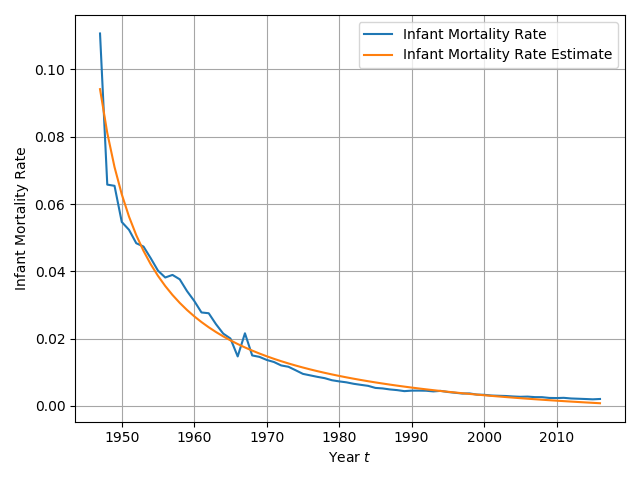
\includegraphics[width=0.50\textwidth]{\FigureDir/mortality/smooth_0/_infant_mortality_rate_predicted.png}
         \end{tabular}
      \end{threeparttable}
   }
\end{figure}

\noindent
I begin the non-infant mortality rate estimation by fitting the yearly distributions using a generalized beta 2 distribution. The pdf for this distribution can be seen in \ref{eq:A.1-3}. This is the same distribution used to fit fertility estimates. I choose to use a generalized beta 2 distribution rather than an exponential, which is what the data appears to follow, because the fit is almost identical but there is no discernable trend in parameter estimates for an exponential distribution but there is a very clear trend for the generalized beta 2 distribution.
\\\\
As with fertility rates, because the generalized beta 2 is a pdf but mortality rates are not a pdf, I also have to add in a scale parameter. I estimate mortality parameters from 1970 to 2014, the same years as for fertility rates.
\\\\
The fit of the model in selected years can be seen in \autoref{fig:\thesubsubsection2}. The estimated distribution has a very close fit to the true data. This is true for all years, unlike the fertility estimates which do not fit the tails properly for recent data.
\\\\
Parameter estimates and their fit over time can be seen in \autoref{fig:\thesubsubsection3}. In order to ensure estimated trends converge over time, I fit these parameter estimates to logistic functions. The logistic function can be seen in \ref{eq:A.1-4}. This is the same distribution used to fit fertility parameters.

\begin{figure}[H]
   \centering
   \caption{\label{fig:\thesubsubsection2}Mortality Estimated by Generalized Beta 2}
   \scalebox{0.61}{
      \begin{threeparttable}
         \begin{tabular}{cc}
            \includegraphics[width=0.50\textwidth]{\FigureDir/mortality/smooth_0/1970.png} &
            \includegraphics[width=0.50\textwidth]{\FigureDir/mortality/smooth_0/1990.png} \\
            \includegraphics[width=0.50\textwidth]{\FigureDir/mortality/smooth_0/2000.png} &
            \includegraphics[width=0.50\textwidth]{\FigureDir/mortality/smooth_0/2014.png}
         \end{tabular}
      \end{threeparttable}
   }
\end{figure}

\begin{figure}[H]
   \centering
   \caption{\label{fig:\thesubsubsection3}Mortality Generalized Beta 2 Parameter Estimates}
   \scalebox{0.61}{
      \begin{threeparttable}
         \begin{tabular}{cc}
            \includegraphics[width=0.50\textwidth]{\FigureDir/mortality/smooth_0/_a_predicted.png} &
            \includegraphics[width=0.50\textwidth]{\FigureDir/mortality/smooth_0/_b_predicted.png} \\
            \includegraphics[width=0.50\textwidth]{\FigureDir/mortality/smooth_0/_p_predicted.png} &
            \includegraphics[width=0.50\textwidth]{\FigureDir/mortality/smooth_0/_q_predicted.png}
         \end{tabular}
      \end{threeparttable}
   }
   \scalebox{0.61}{
      \begin{tabular}{ccc}
         & \includegraphics[width=0.50\textwidth]{\FigureDir/mortality/smooth_0/_scale_predicted.png} &
      \end{tabular}
   }
\end{figure}

\noindent
With the parameters from the logistic function estimated, we can now test the quality of our model fit. Comparisons of the models estimated with true data can be seen in \autoref{fig:\thesubsubsection4}. The first panel shows the trend in true mortality rates from 1970-2014; the second panel shows the trend in model mortality rates from 1970-2014 using the logistic estimates of the generalized beta 2 parameters; the third panel shows the first two trends overlaid, with true data in red and model data in blue; and the fourth panel shows select estimates from the model.
\\\\
From the first three panels, we can see that the model represents the general trends in mortality rates properly. 
\\\\
The fourth panel gives us an indication of how mortality will evolve over time. We can see consistent decline in mortality from 1990 to 2000 to 2014, which follows the same trend as the true data. With our model we now also have the ability to forecast future mortality rates. Our model forecasts that by 2050 mortality rates will continue their trend downward. We also see that the logistic functional form leads to a convergence in mortality rates by 2050 - the estimate for 2100 is almost exactly overlaid with the estimate for 2050.

\begin{figure}[H]
   \centering
   \caption{\label{fig:\thesubsubsection4}Mortality Generalized Beta 2 Model Fit}
   \scalebox{1}{
      \begin{threeparttable}
         \begin{tabular}{cc}
            \includegraphics[width=0.50\textwidth]{\FigureDir/mortality/smooth_0/_aggregate_true.png} &
            \includegraphics[width=0.50\textwidth]{\FigureDir/mortality/smooth_0/_aggregate_predicted.png} \\
            \includegraphics[width=0.50\textwidth]{\FigureDir/mortality/smooth_0/_aggregate_overlay_predicted.png} &
            \includegraphics[width=0.50\textwidth]{\FigureDir/mortality/smooth_0/_2100.png}
         \end{tabular}
      \end{threeparttable}
   }
\end{figure}

% %%%%%%%%%%%%%%%%%%%%%%%%%%%%%%%%%%%%%%%%%%%%%%%%%
% \subsubsection{Appendix - Demographics - Immigration Rates}
% %%%%%%%%%%%%%%%%%%%%%%%%%%%%%%%%%%%%%%%%%%%%%%%%%

\subsubsection{Immigration Rates}

Estimating the evolution of immigration rates over time poses more of a challenge than fertility or mortality rates. While fertility and mortality rates can be estimated using a generalized beta 2 distribution, immigration rates following a distribution that is difficult to model without a mixture method. To get around this, I instead model the evolution in immigration rates for each age. While this no longer allows for the use of a simple distribution and clear parameter evolutions over time for the entire set of data, it seems like a more reasonable way to fit the data than to fit a mixture model with a large number of distributions.
\\\\
To fit the evolution of immigration rates for each age, I estimate the trend from 1997-2014 using linear regression, then forecast using an exponential distribution that matches the slope of the linear regression in 2014 and is assumed to plateau in 15 years at a value 10\% beyond the last value in the data. The exponential I fit can be seen in \ref{eq:A.1-6}:

\begin{equation}
   f(x|a, b, c, d, p, s, \beta_0, \beta_1) = e^{a(x-s)^2 + b(x-s) + c} + p
\end{equation}

\begin{align*}
   s.t. \hspace{5mm} &\left.\pdv{f}{x}\right|_{x=s} = \beta_1 \tag{cond. 1} \label{c1} \\
   &f(s) = \beta_0 + \beta_1 s \tag{cond. 2} \label{c2} \\
   &\left.\pdv{f}{x}\right|_{x=s + 15} \approx 0 \tag{cond. 3} \label{c3} \\
   &f(s + 15) = d \cdot f(s) \tag{cond. 4} \label{c4}
\end{align*}

\noindent
where \(a, b\), and \(c\) are parameters to estimate, \(p\) shifts the curve so we can estimate \(c\) (this is explained in the derivation), \(s\) gives the last year of data, \(\beta_0\) and \(\beta_1\) are the OLS estimates from fitting the data, and we define \(d\) such that

\[
   d = \left\{\begin{matrix}
      0.9 & \text{if} & (\beta < 0 \text{ and } f(s) > 0) \text{ or } (\beta > 0 \text{ and } f(s) < 0) \\
      1.1 & \text{if} & (\beta < 0 \text{ and } f(s) < 0) \text{ or } (\beta > 0 \text{ and } f(s) > 0) \\
      1 & \text{if} & \beta = 0
   \end{matrix}\right.
\]

\noindent
For notational simplicity, I will define \(\beta = \beta_0 + \beta_1s\). We therefore have from \ref{c2} that \(e^c + p = \beta \Leftrightarrow c = \log(\beta - p)\). In order to ensure that we can compute \(c\), we set \(p < \beta\).
\\\\
Using \(\pdv{f}{x} = (2a(x-s) + b)e^{a(x-s)^2 + b(x-s) + c}\) and \ref{c1}, we have \(be^c = \beta_1 \Leftrightarrow b = \frac{\beta_1}{\beta - p}\).
\\\\
From \ref{c3} we have \((2a(15) + b)(f(x+15) - p) \approx 0\). Plugging in the value for \(f(x+15)\) from \ref{c4}, and recalling that \(f(s) = \beta_0 + \beta_1s = \beta\), we have \(\left(2a(15) + \frac{\beta_1}{\beta - p}\right)(d\cdot \beta - g) \approx 0 \Leftrightarrow a \approx \frac{1}{30}\left(\frac{0}{d\cdot\beta-g} - \frac{\beta_1}{\beta - p}\right)\). Because the derivative cannot actually become 0, we can choose a value very close to 0 to estimate this curve numerically. At 2030, we assume that the estimate stays constant for future years.
\\\\
We therefore have the following:
\[
   \left\{
      p < \beta,
      a \approx \frac{1}{30}\left(\frac{0}{d\cdot\beta - g} - \frac{\beta_1}{\beta - p}\right),
      b = \frac{\beta_1}{\beta - p},
      c = \log(\beta - p)
   \right\}
\]
\noindent
where \(\beta = \beta_0 + \beta_1s\).
\\\\
The fit of the model for selected ages can be seen in \autoref{fig:\thesubsubsection1}. Unlike fertility and mortality rates, fertility rates by age appear not to have as predictable a trend. However, the linear regression model with exponential forecasts seems sufficient to have reasonable forecasts for the short term.

\begin{figure}[H]
   \centering
   \caption{\label{fig:\thesubsubsection1}Immigration Estimated by Linear Regression and Forecasted by Exponential}
   \scalebox{0.9}{
      \begin{threeparttable}
         \begin{tabular}{cc}
            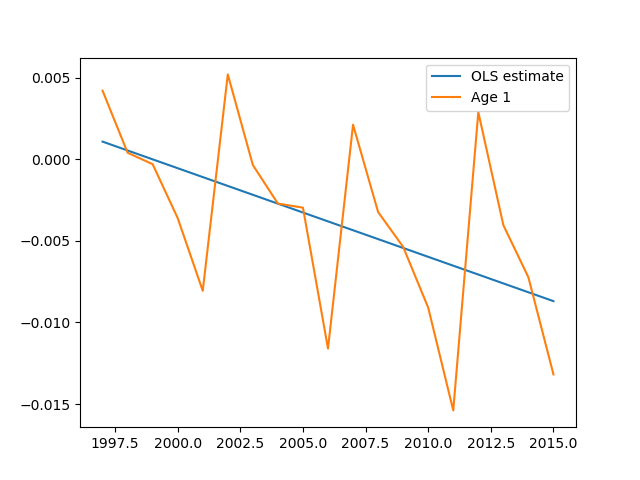
\includegraphics[width=0.50\textwidth]{\FigureDir/immigration/age_forecasts/1.png} &
            \includegraphics[width=0.50\textwidth]{\FigureDir/immigration/age_forecasts/20.png} \\
            \includegraphics[width=0.50\textwidth]{\FigureDir/immigration/age_forecasts/50.png} &
            \includegraphics[width=0.50\textwidth]{\FigureDir/immigration/age_forecasts/90.png}
         \end{tabular}
      \end{threeparttable}
   }
\end{figure}

\noindent
With the parameters from the linear regression and exponential estimated, we can now test the quality of our model fit. Comparisons of the models estimated with true data can be seen in \autoref{fig:\thesubsubsection2}. The first panel shows the trend in true immigration rates from 1997-2014; the second panel shows the trend in model immigration rates from 1997-2014; the third panel shows the first two trends overlaid, with true data in red and model data in blue; and the fourth panel shows select estimates from the model.
\\\\
From the first three panels, we can see that the model represents the general trends in immigration rates properly, although with reduced variance. 
\\\\
The fourth panel gives us an indication of how immigration will evolve over time. We can see consistent decline in immigration from 1990 to 2000 to 2014 for the young and the old, with little change in immigration rates for other ages, which follows the same trend as the true data. With our model we now also have the ability to forecast future immigration rates. Our model forecasts that by 2050 immigration rates will continue their trend downward for the old. In order to prevent population estimates from declining too rapidly I choose to increase immigration rates for the 0 year old population rather than let it continue to decline. Other ages seem to have relatively unchanged immigration rates over time. We can also see that following our construction, we have a convergence in immigration rates by 2030.

\begin{figure}[H]
   \centering
   \caption{\label{fig:\thesubsubsection2}Immigration Estimated by Linear Regression and Forecasted by Exponential}
   \scalebox{1}{
      \begin{threeparttable}
         \begin{tabular}{cc}
            \includegraphics[width=0.50\textwidth]{\FigureDir/immigration/smooth_0/_aggregate_true.png} &
            \includegraphics[width=0.50\textwidth]{\FigureDir/immigration/smooth_0/_aggregate_predicted.png} \\
            \includegraphics[width=0.50\textwidth]{\FigureDir/immigration/smooth_0/_aggregate_overlay_predicted.png} &
            \includegraphics[width=0.50\textwidth]{\FigureDir/immigration/smooth_0/_2100.png}
         \end{tabular}
      \end{threeparttable}
   }
\end{figure}

% %%%%%%%%%%%%%%%%%%%%%%%%%%%%%%%%%%%%%%%%%%%%%%%%%
% \subsubsection{Appendix - Demographics - Population}
% %%%%%%%%%%%%%%%%%%%%%%%%%%%%%%%%%%%%%%%%%%%%%%%%%

\subsubsection{Population}

Using our fertility, mortality, and immigration estimates, we can now use the population evolution described in \ref{eq:A.1-1} and \ref{eq:A.1-2} to forecast future population given an initial year of population data.
\\\\
We will first analyze quality of fit on past data. I test by beginning with 1970 population data and comparing the true population evolution against the population evolution forecasted by the model. Selected years of the transition from 1970 to 2017, the most recent population data, can be seen in \autoref{fig:\thesubsubsection1}. We can see in the first year of the model that there is a slight overestimate of births. This persists over time for this particular cohort, as the mortality rate should not be compensating for this. However, this slight overestimate is actually a rise in population that is is seen to occur just a few years later in the true data, when looking at the figure from 1985. The model does an accurate job of representing the inflection point in population that occurs around 1974 in the real data, and 1972 in the forecast. Looking at the figure from 2000, we can see that the model also accurately fits the inflection point in population around 1997. However, we begin to see that there a few ages where the model is overestimating the population and other ages where it is underestimating the population. The final figure is for 2017. This is 47 years after the start. The model appears to fit the data well and reflects the inflection points in the data. 

\begin{figure}[H]
   \centering
   \caption{\label{fig:\thesubsubsection1}Forecasted vs. True Population}
   \scalebox{1}{
      \begin{threeparttable}
         \begin{tabular}{cc}
            \includegraphics[width=0.50\textwidth]{\FigureDir/population_forecasts/start_1970/1971.png} &
            \includegraphics[width=0.50\textwidth]{\FigureDir/population_forecasts/start_1970/1985.png} \\
            \includegraphics[width=0.50\textwidth]{\FigureDir/population_forecasts/start_1970/2000.png} &
            \includegraphics[width=0.50\textwidth]{\FigureDir/population_forecasts/start_1970/2017.png}
         \end{tabular}
      \end{threeparttable}
   }
\end{figure}

\noindent
Given the model does a good job of fitting historical data, we now move on to forecasting future populations. We can see how population will evolve over time in \autoref{fig:\thesubsubsection2}. The first panel shows the population at select years in the future. These results are rather surprising. We can see that given the forecasts for fertility, mortality, and immigration rates, the population in Japan is not sustainable. According to this model, by the year 2500 the population will have effectively disappeared. This result should caution the user of this model - it can lead to counterintuitive and unreasonable results. However, without another model to use in its place, this model is used for the estimation in this paper.
\\\\
The second panel shows the distribution of the population at select years in the future. We can see that over time, the modal age of the population increases until it peaks at around 75 years old. While this result indicates Japan faces a massive hurdle with its aging population, it should be taken with a grain of salt considering that the model estimates that by the time the demographic distribution reaches this point, the population will be effectively 0.

\begin{figure}[H]
   \centering
   \caption{\label{fig:\thesubsubsection2}Forecasted Population and Population Distribution}
   \scalebox{1}{
      \begin{threeparttable}
         \begin{tabular}{cc}
            \includegraphics[width=0.50\textwidth]{\FigureDir/population_forecasts/start_2017/predicted_basic.png} & \includegraphics[width=0.50\textwidth]{\FigureDir/population_forecasts/start_2017/predicted_proportion_basic.png} \\
            \includegraphics[width=0.50\textwidth]{\FigureDir/population_forecasts/start_2017/predicted_parametric.png} & \includegraphics[width=0.50\textwidth]{\FigureDir/population_forecasts/start_2017/predicted_proportion_parametric.png} \\
            \includegraphics[width=0.50\textwidth]{\FigureDir/population_forecasts/start_2017/predicted_alt.png} & \includegraphics[width=0.50\textwidth]{\FigureDir/population_forecasts/start_2017/predicted_proportion_alt.png}
         \end{tabular}
      \end{threeparttable}
   }
\end{figure}

% %%%%%%%%%%%%%%%%%%%%%%%%%%%%%%%%%%%%%%%%%%%%%%%%%
% \subsection{Appendix - Results}
% %%%%%%%%%%%%%%%%%%%%%%%%%%%%%%%%%%%%%%%%%%%%%%%%%

\subsection{Results}

% %%%%%%%%%%%%%%%%%%%%%%%%%%%%%%%%%%%%%%%%%%%%%%%%%
% \subsubsection{Appendix - Results - Steady State Results}
% %%%%%%%%%%%%%%%%%%%%%%%%%%%%%%%%%%%%%%%%%%%%%%%%%

\subsubsection{Steady State Results}

\begin{figure}[H]
   \caption{\label{fig:\thesubsubsection1}Steady State Consumption and Savings}
   \begin{subfigure}{0.5\textwidth}
      \centering
      \includegraphics[width=\textwidth]{\SSDir/static/images/SS_bc.png}
      \caption{Static Demographics}
   \end{subfigure}%
   ~
   \begin{subfigure}{0.5\textwidth}
      \centering
      \includegraphics[width=\textwidth]{\SSDir/dynamic_partial/images/SS_bc.png}
      \caption{Partial-Dynamic Demographics}
   \end{subfigure}
   \newline
   \begin{subfigure}{0.5\textwidth}
      \centering
      \includegraphics[width=\textwidth]{\SSDir/dynamic_full/images/SS_bc.png}
      \caption{Full-Dynamic Demographics}
   \end{subfigure}%
   ~
   \begin{subfigure}{0.5\textwidth}
      \centering
      \includegraphics[width=\textwidth]{\SSDir/dynamic_full_alternate/images/SS_bc.png}
      \caption{Alternate Full-Dynamic Demographics}
   \end{subfigure}
\end{figure}

\begin{figure}[H]
   \caption{\label{fig:\thesubsubsection1}Steady State Labor Supply}
   \begin{subfigure}{0.5\textwidth}
      \centering
      \includegraphics[width=\textwidth]{\SSDir/static/images/SS_n.png}
      \caption{Static Demographics}
   \end{subfigure}%
   ~
   \begin{subfigure}{0.5\textwidth}
      \centering
      \includegraphics[width=\textwidth]{\SSDir/dynamic_partial/images/SS_n.png}
      \caption{Partial-Dynamic Demographics}
   \end{subfigure}
   \newline
   \begin{subfigure}{0.5\textwidth}
      \centering
      \includegraphics[width=\textwidth]{\SSDir/dynamic_full/images/SS_n.png}
      \caption{Full-Dynamic Demographics}
   \end{subfigure}%
   ~
   \begin{subfigure}{0.5\textwidth}
      \centering
      \includegraphics[width=\textwidth]{\SSDir/dynamic_full_alternate/images/SS_n.png}
      \caption{Alternate Full-Dynamic Demographics}
   \end{subfigure}
\end{figure}

% %%%%%%%%%%%%%%%%%%%%%%%%%%%%%%%%%%%%%%%%%%%%%%%%%
% \subsubsection{Appendix - Results - Time Path Results}
% %%%%%%%%%%%%%%%%%%%%%%%%%%%%%%%%%%%%%%%%%%%%%%%%%

\subsubsection{Time Path Results}

\begin{figure}[H]
   \caption{\label{fig:\thesubsubsection1}Time Path of Total Bequests \(\hat{BQ}_t\)}
   \begin{subfigure}{0.5\textwidth}
      \centering
      \includegraphics[width=\textwidth]{\TPDir/static/images/TP_BQ_path.png}
      \caption{Static Demographics}
   \end{subfigure}%
   ~
   \begin{subfigure}{0.5\textwidth}
      \centering
      \includegraphics[width=\textwidth]{\TPDir/dynamic_partial/images/TP_BQ_path.png}
      \caption{Partial-Dynamic Demographics}
   \end{subfigure}
   \newline
   \begin{subfigure}{0.5\textwidth}
      \centering
      \includegraphics[width=\textwidth]{\TPDir/dynamic_full/images/TP_BQ_path.png}
      \caption{Full-Dynamic Demographics}
   \end{subfigure}%
   ~
   \begin{subfigure}{0.5\textwidth}
      \centering
      \includegraphics[width=\textwidth]{\TPDir/dynamic_full_alternate/images/TP_BQ_path.png}
      \caption{Alternate Full-Dynamic Demographics}
   \end{subfigure}
\end{figure}

\begin{figure}[H]
   \caption{\label{fig:\thesubsubsection1}Time Path of Individual Savings \(b_{s,t}\)}
   \begin{subfigure}{0.5\textwidth}
      \centering
      \includegraphics[width=\textwidth]{\TPDir/static/images/TP_bs_path.png}
      \caption{Static Demographics}
   \end{subfigure}%
   ~
   \begin{subfigure}{0.5\textwidth}
      \centering
      \includegraphics[width=\textwidth]{\TPDir/dynamic_partial/images/TP_bs_path.png}
      \caption{Partial-Dynamic Demographics}
   \end{subfigure}
   \newline
   \begin{subfigure}{0.5\textwidth}
      \centering
      \includegraphics[width=\textwidth]{\TPDir/dynamic_full/images/TP_bs_path.png}
      \caption{Full-Dynamic Demographics}
   \end{subfigure}%
   ~
   \begin{subfigure}{0.5\textwidth}
      \centering
      \includegraphics[width=\textwidth]{\TPDir/dynamic_full_alternate/images/TP_bs_path.png}
      \caption{Alternate Full-Dynamic Demographics}
   \end{subfigure}
\end{figure}

\begin{figure}[H]
   \caption{\label{fig:\thesubsubsection1}Time Path of Aggregate Consumption \(\hat{C}_t\)}
   \begin{subfigure}{0.5\textwidth}
      \centering
      \includegraphics[width=\textwidth]{\TPDir/static/images/TP_C_path.png}
      \caption{Static Demographics}
   \end{subfigure}%
   ~
   \begin{subfigure}{0.5\textwidth}
      \centering
      \includegraphics[width=\textwidth]{\TPDir/dynamic_partial/images/TP_C_path.png}
      \caption{Partial-Dynamic Demographics}
   \end{subfigure}
   \newline
   \begin{subfigure}{0.5\textwidth}
      \centering
      \includegraphics[width=\textwidth]{\TPDir/dynamic_full/images/TP_C_path.png}
      \caption{Full-Dynamic Demographics}
   \end{subfigure}%
   ~
   \begin{subfigure}{0.5\textwidth}
      \centering
      \includegraphics[width=\textwidth]{\TPDir/dynamic_full_alternate/images/TP_C_path.png}
      \caption{Alternate Full-Dynamic Demographics}
   \end{subfigure}
\end{figure}

\begin{figure}[H]
   \caption{\label{fig:\thesubsubsection1}Time Path of Individual Consumption \(\hat{c}_{s,t}\)}
   \begin{subfigure}{0.5\textwidth}
      \centering
      \includegraphics[width=\textwidth]{\TPDir/static/images/TP_cs_path.png}
      \caption{Static Demographics}
   \end{subfigure}%
   ~
   \begin{subfigure}{0.5\textwidth}
      \centering
      \includegraphics[width=\textwidth]{\TPDir/dynamic_partial/images/TP_cs_path.png}
      \caption{Partial-Dynamic Demographics}
   \end{subfigure}
   \newline
   \begin{subfigure}{0.5\textwidth}
      \centering
      \includegraphics[width=\textwidth]{\TPDir/dynamic_full/images/TP_cs_path.png}
      \caption{Full-Dynamic Demographics}
   \end{subfigure}%
   ~
   \begin{subfigure}{0.5\textwidth}
      \centering
      \includegraphics[width=\textwidth]{\TPDir/dynamic_full_alternate/images/TP_cs_path.png}
      \caption{Alternate Full-Dynamic Demographics}
   \end{subfigure}
\end{figure}

\begin{figure}[H]
   \caption{\label{fig:\thesubsubsection1}Time Path of Aggregate Investment \(\hat{I}_t\)}
   \begin{subfigure}{0.5\textwidth}
      \centering
      \includegraphics[width=\textwidth]{\TPDir/static/images/TP_I_path.png}
      \caption{Static Demographics}
   \end{subfigure}%
   ~
   \begin{subfigure}{0.5\textwidth}
      \centering
      \includegraphics[width=\textwidth]{\TPDir/dynamic_partial/images/TP_I_path.png}
      \caption{Partial-Dynamic Demographics}
   \end{subfigure}
   \newline
   \begin{subfigure}{0.5\textwidth}
      \centering
      \includegraphics[width=\textwidth]{\TPDir/dynamic_full/images/TP_I_path.png}
      \caption{Full-Dynamic Demographics}
   \end{subfigure}%
   ~
   \begin{subfigure}{0.5\textwidth}
      \centering
      \includegraphics[width=\textwidth]{\TPDir/dynamic_full_alternate/images/TP_I_path.png}
      \caption{Alternate Full-Dynamic Demographics}
   \end{subfigure}
\end{figure}

\begin{figure}[H]
   \caption{\label{fig:\thesubsubsection1}Time Path of Aggregate Capital \(\hat{K}_t\)}
   \begin{subfigure}{0.5\textwidth}
      \centering
      \includegraphics[width=\textwidth]{\TPDir/static/images/TP_K_path.png}
      \caption{Static Demographics}
   \end{subfigure}%
   ~
   \begin{subfigure}{0.5\textwidth}
      \centering
      \includegraphics[width=\textwidth]{\TPDir/dynamic_partial/images/TP_K_path.png}
      \caption{Partial-Dynamic Demographics}
   \end{subfigure}
   \newline
   \begin{subfigure}{0.5\textwidth}
      \centering
      \includegraphics[width=\textwidth]{\TPDir/dynamic_full/images/TP_K_path.png}
      \caption{Full-Dynamic Demographics}
   \end{subfigure}%
   ~
   \begin{subfigure}{0.5\textwidth}
      \centering
      \includegraphics[width=\textwidth]{\TPDir/dynamic_full_alternate/images/TP_K_path.png}
      \caption{Alternate Full-Dynamic Demographics}
   \end{subfigure}
\end{figure}

\begin{figure}[H]
   \caption{\label{fig:\thesubsubsection1}Time Path of Aggregate Labor Supply \(\hat{L}_t\)}
   \begin{subfigure}{0.5\textwidth}
      \centering
      \includegraphics[width=\textwidth]{\TPDir/static/images/TP_L_path.png}
      \caption{Static Demographics}
   \end{subfigure}%
   ~
   \begin{subfigure}{0.5\textwidth}
      \centering
      \includegraphics[width=\textwidth]{\TPDir/dynamic_partial/images/TP_L_path.png}
      \caption{Partial-Dynamic Demographics}
   \end{subfigure}
   \newline
   \begin{subfigure}{0.5\textwidth}
      \centering
      \includegraphics[width=\textwidth]{\TPDir/dynamic_full/images/TP_L_path.png}
      \caption{Full-Dynamic Demographics}
   \end{subfigure}%
   ~
   \begin{subfigure}{0.5\textwidth}
      \centering
      \includegraphics[width=\textwidth]{\TPDir/dynamic_full_alternate/images/TP_L_path.png}
      \caption{Alternate Full-Dynamic Demographics}
   \end{subfigure}
\end{figure}

\begin{figure}[H]
   \caption{\label{fig:\thesubsubsection1}Time Path of Individual Labor Supply \(n_{s,t}\)}
   \begin{subfigure}{0.5\textwidth}
      \centering
      \includegraphics[width=\textwidth]{\TPDir/static/images/TP_ns_path.png}
      \caption{Static Demographics}
   \end{subfigure}%
   ~
   \begin{subfigure}{0.5\textwidth}
      \centering
      \includegraphics[width=\textwidth]{\TPDir/dynamic_partial/images/TP_ns_path.png}
      \caption{Partial-Dynamic Demographics}
   \end{subfigure}
   \newline
   \begin{subfigure}{0.5\textwidth}
      \centering
      \includegraphics[width=\textwidth]{\TPDir/dynamic_full/images/TP_ns_path.png}
      \caption{Full-Dynamic Demographics}
   \end{subfigure}%
   ~
   \begin{subfigure}{0.5\textwidth}
      \centering
      \includegraphics[width=\textwidth]{\TPDir/dynamic_full_alternate/images/TP_ns_path.png}
      \caption{Alternate Full-Dynamic Demographics}
   \end{subfigure}
\end{figure}

\begin{figure}[H]
   \caption{\label{fig:\thesubsubsection1}Time Path of Net Exports \(\hat{NX}_t\)}
   \begin{subfigure}{0.5\textwidth}
      \centering
      \includegraphics[width=\textwidth]{\TPDir/static/images/TP_NX_path.png}
      \caption{Static Demographics}
   \end{subfigure}%
   ~
   \begin{subfigure}{0.5\textwidth}
      \centering
      \includegraphics[width=\textwidth]{\TPDir/dynamic_partial/images/TP_NX_path.png}
      \caption{Partial-Dynamic Demographics}
   \end{subfigure}
   \newline
   \begin{subfigure}{0.5\textwidth}
      \centering
      \includegraphics[width=\textwidth]{\TPDir/dynamic_full/images/TP_NX_path.png}
      \caption{Full-Dynamic Demographics}
   \end{subfigure}%
   ~
   \begin{subfigure}{0.5\textwidth}
      \centering
      \includegraphics[width=\textwidth]{\TPDir/dynamic_full_alternate/images/TP_NX_path.png}
      \caption{Alternate Full-Dynamic Demographics}
   \end{subfigure}
\end{figure}

\begin{figure}[H]
   \caption{\label{fig:\thesubsubsection1}Time Path of Interest Rate \(r_t\)}
   \begin{subfigure}{0.5\textwidth}
      \centering
      \includegraphics[width=\textwidth]{\TPDir/static/images/TP_r_path.png}
      \caption{Static Demographics}
   \end{subfigure}%
   ~
   \begin{subfigure}{0.5\textwidth}
      \centering
      \includegraphics[width=\textwidth]{\TPDir/dynamic_partial/images/TP_r_path.png}
      \caption{Partial-Dynamic Demographics}
   \end{subfigure}
   \newline
   \begin{subfigure}{0.5\textwidth}
      \centering
      \includegraphics[width=\textwidth]{\TPDir/dynamic_full/images/TP_r_path.png}
      \caption{Full-Dynamic Demographics}
   \end{subfigure}%
   ~
   \begin{subfigure}{0.5\textwidth}
      \centering
      \includegraphics[width=\textwidth]{\TPDir/dynamic_full_alternate/images/TP_r_path.png}
      \caption{Alternate Full-Dynamic Demographics}
   \end{subfigure}
\end{figure}

\begin{figure}[H]
   \caption{\label{fig:\thesubsubsection1}Time Path of Wage \(\hat{w}_t\)}
   \begin{subfigure}{0.5\textwidth}
      \centering
      \includegraphics[width=\textwidth]{\TPDir/static/images/TP_w_path.png}
      \caption{Static Demographics}
   \end{subfigure}%
   ~
   \begin{subfigure}{0.5\textwidth}
      \centering
      \includegraphics[width=\textwidth]{\TPDir/dynamic_partial/images/TP_w_path.png}
      \caption{Partial-Dynamic Demographics}
   \end{subfigure}
   \newline
   \begin{subfigure}{0.5\textwidth}
      \centering
      \includegraphics[width=\textwidth]{\TPDir/dynamic_full/images/TP_w_path.png}
      \caption{Full-Dynamic Demographics}
   \end{subfigure}%
   ~
   \begin{subfigure}{0.5\textwidth}
      \centering
      \includegraphics[width=\textwidth]{\TPDir/dynamic_full_alternate/images/TP_w_path.png}
      \caption{Alternate Full-Dynamic Demographics}
   \end{subfigure}
\end{figure}

\begin{figure}[H]
   \caption{\label{fig:\thesubsubsection1}Time Path of Aggregate Output \(\hat{Y}_t\)}
   \begin{subfigure}{0.5\textwidth}
      \centering
      \includegraphics[width=\textwidth]{\TPDir/static/images/TP_Y_path.png}
      \caption{Static Demographics}
   \end{subfigure}%
   ~
   \begin{subfigure}{0.5\textwidth}
      \centering
      \includegraphics[width=\textwidth]{\TPDir/dynamic_partial/images/TP_Y_path.png}
      \caption{Partial-Dynamic Demographics}
   \end{subfigure}
   \newline
   \begin{subfigure}{0.5\textwidth}
      \centering
      \includegraphics[width=\textwidth]{\TPDir/dynamic_full/images/TP_Y_path.png}
      \caption{Full-Dynamic Demographics}
   \end{subfigure}%
   ~
   \begin{subfigure}{0.5\textwidth}
      \centering
      \includegraphics[width=\textwidth]{\TPDir/dynamic_full_alternate/images/TP_Y_path.png}
      \caption{Alternate Full-Dynamic Demographics}
   \end{subfigure}
\end{figure}

\end{appendices}

\end{document}
